\documentclass[a4paper, titlepage, oneside]{article}
\usepackage[vmargin=2cm,hmargin=2cm]{geometry}
\usepackage{amsmath,amssymb} % mathematical markup
\usepackage{graphicx,epstopdf,listings,csvsimple,float,xcolor}
\usepackage[allcolors=blue,colorlinks=true]{hyperref}
\usepackage{multicol}
\usepackage{gensymb}
\usepackage{wasysym}
\usepackage[backend = biber, style = authoryear, alldates = iso8601]{biblatex}


% listings, xcolor
\lstset{language=Matlab,
    commentstyle=\color{gray}\textit,
    stringstyle=\color{purple},
    showstringspaces=false,
    numbers=left,
    breaklines=true,
    breakatwhitespace=true,
    aboveskip=0pt,
    belowskip=20pt}

% geometry  : page margins
% amsmath : maths
% amssymb : maths
% graphicx  : \includegraphic
% epstopdf  : use of eps files in document
% hyperref  : in-document links
% listings  : import external code
% csvsimple : import csv tables
% float   : float graphics
% xcolor  : use colour formatting
% gensymb : \degree, \celsius, \micro, \ohm
% wasysym : \astrosun (conflict with amssymb)
% biblatex : bibliography

% Bibliography setup
\renewcommand{\nameyeardelim}{\addcomma\addspace} % Change delimiter for in-line citations to include a comma
\addbibresource{group-report.bib}

% Custom commands
\newcommand{\elem}[2]{\textsuperscript{#1}{#2}}
\newcommand{\e}[1]{\ensuremath{\times 10^{#1}}}

% Document proper
\begin{document}
\title{\textbf{Searching for molecular gas towards TeV gamma-ray sources: Analysing 3D data cubes of the molecular gas tracer carbon monoxide with images from the HESS gamma-ray telescopes.}}
\author{A.~K. Child \and C.~M. Roe-Simons \and K.~T. Leaver \and H.~D. Poulter \and R.~M. Harvey}
\maketitle
\date{} %Leave blank to print no date, or you can type in the desired date

\setcounter{page}{1}
\pagenumbering{roman}
\numberwithin{equation}{section}

\tableofcontents

\clearpage
\setcounter{page}{1}
\pagenumbering{arabic}

\begin{center}
{\LARGE \textbf{Searching for molecular gas towards TeV gamma-ray sources: Analysing 3D data cubes of the molecular gas tracer carbon monoxide with images from the HESS gamma-ray telescopes.}}

\vspace{1.5em}

\textsc{A.~K. Child\footnote{Featured Telescopes} \quad C.~M. Roe-Simons\footnote{Cosmic Ray Sources} \quad K.~T. Leaver\footnote{CO, \elem{13}{CO} as tracers} \quad H.~D. Poulter\footnote{Galactic Rotation} \quad R.~M. Harvey\footnote{Molecular Clouds and CR interactions}}
\end{center}

\vspace{2em}

\begin{minipage}{0.93\textwidth}
\begin{abstract}
This report is about finding the TeV sources and molecular clouds associated with such sources. It beings with a brief overview of the types of physical and astronomical concepts behind the science that has been used in writing up the report and making the conclusions. Bro!
\end{abstract}
\end{minipage}

\vspace{2.5em}

\begin{multicols}{2}
\section{Introduction}
Words words words, quick run-down of gamma rays and really high ones, just pretty much do a Gavin and copy stuff from Gavin's slides and so on and so forth.

\section{Theory}
Theory stuff goes in here, including but not limited to:
\begin{itemize}
\item Cosmic ray sources
\item Large molecular clouds, and their interactions with CRs
\item CO \& 13CO as tracers
\item Telescope information/general data stuff?
\item Galactic rotation/Doppler shift in Mopra data
\end{itemize}
Fun!

\subsection{Cosmic Ray Sources}
Go Coen! Goen! Wow that was awful!

\subsection{Molecular Clouds and CR interactions}
Go Reece!  Yeah, it's a fun time to be alive! Being like the most bitsh, my ponk can rock stock and frocks.!!

Hi hello yes here is an example of a thing I will reference. \parencite{rmp1}

\subsection{CO, \elem{13}{CO} as tracers}
Kyle is going the extra mile in style! Friend, you have a good plan to make the works go forwards! More words just to make a larger paragraph!

\subsection{Featured Telescopes}
Alisha ain't no child, no siree! I ran out of shitty announcer puns, forgive me! Tele-no-scope 360 xboxs swag!!!

\subsection{Galactic Rotation}
It's a me, shitty mc fuckers, ready to make panties wet (or dicks erect, i don't discriminate here everyone's welcome) with my amazing diagram! This is literally the only thing that will be featured in this section! Just a huge-ass diagram is all anyone ever wanted!!

\begin{figure}[H]
\centering
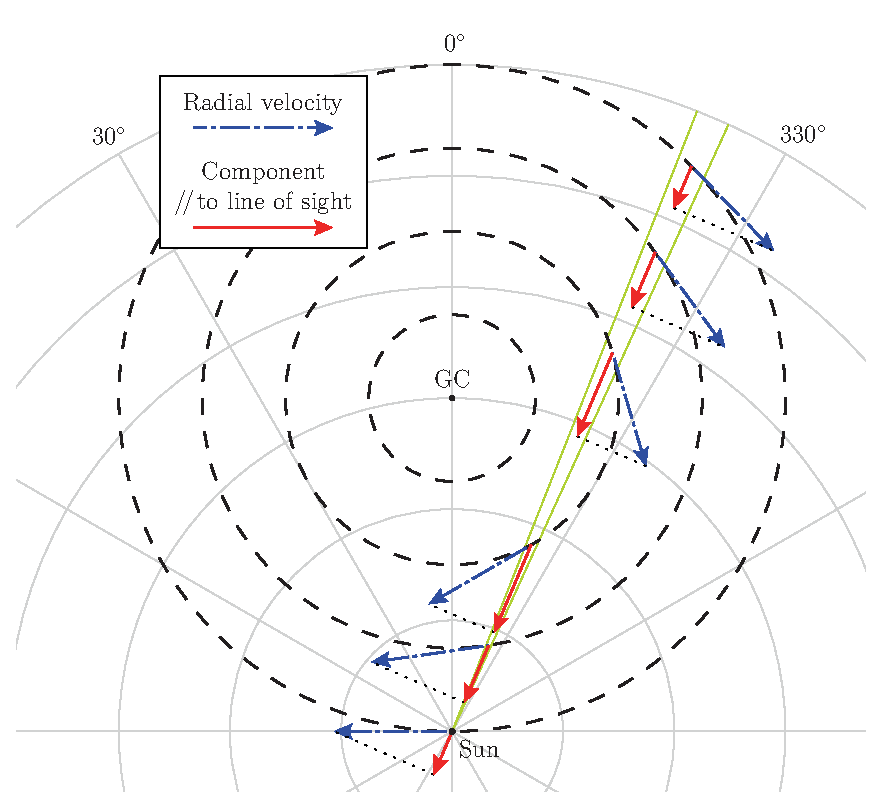
\includegraphics[width=8cm]{figures/galactic-rotation}
\caption{Galactic rotation showing Doppler shifts}
\label{fig:gal-rot}
\end{figure}

\section{Data Analysis}
Data analysis is coming first. We talk about many things including how we managed to reduce the nouse in the \texttt{.fits} files we used to make the analysis. Yeas!

\subsection{Noise Analsyis}
Yes, keem em cumming!!

\section{Results \& Discussion}
This is where we talk aout all the resuts we get from our data analysis, probably a good idea to cover the data analysis first and all of that so that way things make more sense here. Results should relly not even be in here lel.

\subsection{Source Candidates}
Here are some of the candidates for the gamma ray sources observed.

\subsubsection{HESS J1632-479}
Here are the things for this source. Probably include a picture of the source just as a nice ``here is thing''.

\section{Conclusion}
Bitch, we concluding now, making the statements that make a conclusion possible to be made with the words and the mouth. Bitch, we're flawless give us good grades.
\end{multicols}

\printbibliography[heading=bibintoc]

\end{document}